% =====================================================================
% Nine Algorithms, One Ceiling
% A Diagnostic Study of Résumé–Job-Description Fit Prediction
%
% BUILD:
%     pdflatex paper && bibtex paper && pdflatex paper && pdflatex paper
%
% NOTE: this source has NOT been compile-tested — no LaTeX toolchain was
% available on the machine it was written on. Expect to fix minor issues
% (most likely: a missing package on your distribution, or float
% placement). The content is complete and matches PAPER.md exactly.
%
% VENUE SWAP:
%   arXiv / generic (current): \documentclass[11pt]{article} + geometry
%   IEEE conference or Access: replace the two lines marked [CLASS] with
%       \documentclass[conference]{IEEEtran}      % or [journal]
%     and delete the \usepackage{geometry} line and the \affil lines,
%     using IEEEtran's \author{\IEEEauthorblockN{...}} form instead.
%   ACM (FAccT etc.):          \documentclass[sigconf]{acmart}
% =====================================================================

\documentclass[11pt]{article}                      % [CLASS]
\usepackage[margin=1in]{geometry}                  % [CLASS] delete for IEEEtran

\usepackage[utf8]{inputenc}
\usepackage[T1]{fontenc}
\usepackage{lmodern}
\usepackage{amsmath,amssymb}
\usepackage{booktabs}
\usepackage{graphicx}
\usepackage{caption}
\usepackage{multirow}
\usepackage{array}
\usepackage{url}
\usepackage[hidelinks]{hyperref}
\usepackage{microtype}

\graphicspath{{figures/}}

% Compact table font so the wide results tables fit the text block.
\newcommand{\tabfont}{\footnotesize}

\title{\textbf{Nine Algorithms, One Ceiling:\\
A Diagnostic Study of Résumé--Job-Description Fit Prediction}}

% ---------------------------------------------------------------------
% TODO(author): replace the institution placeholder below before
% submission. It was deliberately left unfilled rather than guessed.
% ---------------------------------------------------------------------
\author{Devesh S V\\
  Department of Computer Science and Engineering\\
  \textit{[INSTITUTION --- TO COMPLETE]}\\
  \texttt{deveshsv.386@gmail.com}}

\date{}

\begin{document}
\maketitle

\begin{abstract}
Multi-algorithm comparisons are a staple of applied machine learning and are
routinely reported without grouped cross-validation, significance testing, or any
check that the benchmark rewards the capability its name implies. We conduct one
carefully on a public résumé--job-description fit benchmark (7{,}910 pairs over
643 résumés and 351 postings), and report what the care reveals.

Nine classifiers spanning six model families, evaluated under 10-fold
cross-validation grouped by job posting with per-fold leakage controls, converge
into a band 0.031 AUROC wide; after Holm--Bonferroni correction the leading model
is statistically indistinguishable from all four tree ensembles tested. To
establish that this null is informative rather than underpowered, we run the
identical protocol on a synthetic control with a pre-specified generative process
and a known Bayes ceiling, where it separates the same nine models decisively
(Friedman $p = 3.7 \times 10^{-9}$, against $6.5 \times 10^{-6}$ on the real
task).

Changing the representation moves performance roughly twice as far as changing
the algorithm. A probe that never sees the job posting reaches 0.660 AUROC ---
87\% of the best model's score --- which initially suggested to us that the
benchmark's labels were not relational. Two experiments refute that reading:
80.6\% of label variance is within-résumé, and withholding every test résumé from
training does not degrade performance.

What survives is a decoupling. Moving to a 1536-dimensional interaction encoding
gains 0.041 pooled AUROC and 0.047 between-résumé ranking accuracy, while
within-résumé ranking --- which cancels résumé identity exactly and therefore
isolates matching --- changes by $-0.009$ ($p = 0.45$). The pooled metric sums two
capabilities, ranking candidates and matching candidates to roles, and moved
because the easier one moved.

We propose the within-query ranking statistic as a routine companion to pooled
metrics for any paired benchmark with a recurring entity: it needs no additional
labels, costs one pass over predictions already computed, and has a fixed null of
0.5. For algorithmic hiring it is the measurement that separates a system that
ranks matches from one that ranks people. All code, per-fold results, and figures
accompany this paper.
\end{abstract}

\noindent\textbf{Keywords:} model comparison, benchmark critique, data leakage,
cross-validation, statistical power, algorithmic hiring, résumé matching,
negative results

\section{Introduction}

A recurring pattern in applied machine learning is the model bake-off: several
classifiers are trained on one dataset, a table of scores is reported, and the
largest number is declared the best method for the task. The pattern is routine
enough that its preconditions are rarely stated, let alone checked. Three of them
matter.

The first is that the evaluation protocol controls the leakage paths the dataset
actually contains. The second is that reported differences exceed what
fold-to-fold variation would produce by chance. The third, and the subject of
this paper, is that \textbf{the quantity the benchmark rewards is the quantity
the task is named for}.

The third precondition can fail while the first two hold, and it fails quietly. A
benchmark may contain genuine signal, reward genuine learning, and still direct
effort somewhere other than the capability it advertises --- because a shortcut is
available that the pooled metric cannot distinguish from the real thing. No
amount of care about splits or significance detects this, since both are computed
on the same pooled metric that conflates the two.

We work the problem through on a concrete, publicly available benchmark. The task
is résumé--job-description fit: given a résumé and a job posting, predict whether
the pair is a match. It has obvious commercial application, a public dataset with
over a thousand downloads, and the shape of a problem for which model selection
ought to matter.

We first compare nine classifiers spanning six model families under a protocol
built to make the comparison decidable --- grouped cross-validation, per-fold
leakage controls, non-parametric significance testing, and measured efficiency.
The nine converge into a band roughly three percentage points of AUROC wide, and
after multiplicity correction the leader is statistically indistinguishable from
every tree ensemble in the study. Because a null result of that shape has two
explanations that a table cannot separate --- the algorithms genuinely do not
differ, or the study cannot tell --- we run the identical protocol on a synthetic
task with a pre-specified generative process and a known noise ceiling. There it
separates the same nine models decisively. The null is a property of the task,
not of the study.

Having established that algorithm choice is not the bottleneck, we vary the
representation instead, including two probes constructed so that they
\emph{cannot} be matching: one never sees the job posting, the other never sees
the résumé. The one that never sees the posting reaches 87\% of the best model's
AUROC.

That result initially suggested to us that the benchmark's labels were not
relational at all. \textbf{A direct test refutes it.} Decomposing label variance
shows that 80.6\% is \emph{within}-résumé --- the same résumé labelled fit for one
posting and not for another --- and a ranking test restricted to pairs drawn from a
single résumé, which cancels résumé identity exactly, shows models performing
well above chance (0.633, $p < 10^{-65}$). Genuine matching signal exists, and
models capture some of it.

The finding that survives is narrower and, we think, more useful. Moving from ten
engineered features to a 1536-dimensional interaction encoding buys 0.041 AUROC
on the pooled metric and 0.047 on between-résumé ranking, while producing
\textbf{no measurable change in within-résumé matching} ($-0.009$, $p = 0.45$).
What the pooled metric recorded as a clear improvement was, so far as we can
measure, an improvement at ranking résumés against one another rather than at
matching. On this benchmark, progress up the leaderboard and progress at the task
can come apart --- and the pooled metric cannot show you which one you bought.

\subsection{Contributions}

\begin{enumerate}
\item \textbf{A within-query ranking diagnostic} (\S\ref{sec:matching}) that
separates matching ability from entity-level quality on any paired benchmark
where one side of the pair recurs. It requires no additional labels, costs one
pass over existing predictions, and is the only measurement here that
distinguishes the two capabilities. We argue it should accompany pooled metrics
as standard practice for matching tasks.

\item \textbf{A demonstration that pooled score and matching ability can be
decoupled} (\S\ref{sec:ablation}, \S\ref{sec:matching}): a representation change
worth $+0.041$ pooled AUROC delivers no measurable within-query improvement.

\item \textbf{A statistically disciplined nine-algorithm comparison} on a public
résumé--fit benchmark, using grouped cross-validation, per-fold leakage controls,
Friedman testing, and Holm-corrected pairwise Wilcoxon tests
(\S\ref{sec:protocol}, \S\ref{sec:converge}). We are not aware of a prior
comparison on this dataset that reports fold variance or any significance test.

\item \textbf{A synthetic positive control establishing the protocol's
statistical power} (\S\ref{sec:control}, \S\ref{sec:power}), converting an
ambiguous null into an informative one. We argue this should be standard whenever
a comparison reports no significant difference.

\item \textbf{A representation ablation with one-sided probes}
(\S\ref{sec:ablation}) quantifying how much of the benchmark's score is reachable
without seeing one side of the pair at all.

\item \textbf{Robustness analyses against the three most natural objections}
(\S\ref{sec:robust}) --- that the split still permits leakage, that binarising a
three-class label destroyed the relational signal, and that the models were left
untuned. An equal-budget nested search moves no model more than $+0.0077$ AUROC
and leaves the leader separating from \emph{fewer} rivals, not more. Also here:
generalising to an unseen \emph{posting} is harder than to an unseen
\emph{candidate}, which is the condition every new job requisition presents.

\item \textbf{Efficiency measurements} (\S\ref{sec:efficiency}) showing
predictive quality and computational cost are decoupled here across three orders
of magnitude in inference latency and nearly five in model size.

\item \textbf{A provenance finding about the benchmark}
(\S\ref{sec:provenance}): it is in active use and carries no description,
licence, citation, or documented labelling procedure.

\item \textbf{A survey of the replication landscape}
(\S\ref{sec:noreplication}) showing that no public résumé--fit corpus currently
qualifies as an independent replication target --- the largest alternative shares
100\% of its documents with the corpus under study while reporting 0\% exact-pair
overlap, and the genuinely independent ones pair each résumé with exactly one
posting. We give the normalisation procedure that exposes this class of
contamination, which raw-text hashing misses.
\end{enumerate}

We note explicitly that contribution 2 corrects our own initial hypothesis, which
the experiment in \S\ref{sec:matching} was designed to test and did not support.
We report the sequence because the diagnostic's value is precisely that it was
capable of overturning the conclusion we expected.

All code, per-fold results, and figures accompany this paper; every number is
reproducible from a single command per experiment (Appendix~\ref{sec:repro}).

\section{Related Work}

\paragraph{Model-comparison critiques.}
The closest methodological ancestors of this paper are studies that re-ran
published comparisons under controlled protocols and found the reported progress
did not survive. Ferrari Dacrema, Cremonesi, and
Jannach~\cite{dacrema2019progress} examined eighteen neural recommendation
methods from top-tier venues, could reproduce only seven with reasonable effort,
and found six of those seven were often outperformed by comparably simple
heuristic baselines --- a result that took the RecSys 2019 best-paper award and
reframed a subfield's sense of its own progress. Musgrave, Belongie, and
Lim~\cite{musgrave2020reality} performed the analogous exercise for deep metric
learning and attributed apparent gains to inconsistent experimental practice
rather than to method quality. Our contribution sits in this tradition but
differs in target: rather than showing that a complex method fails to beat a
simple one, we show that on this benchmark \emph{no} method separates from any
other, and then trace why.

\paragraph{Statistical protocol for comparing classifiers.}
Dem\v{s}ar~\cite{demsar2006statistical} is the standard reference for comparing
multiple classifiers, recommending the Friedman test with post-hoc procedures
over repeated parametric tests, and cautioning specifically against reading a
ranking off raw score differences. We follow that protocol. Nadeau and
Bengio~\cite{nadeau2003inference} show that naive variance estimates over
overlapping cross-validation folds understate variability, so a difference that
appears significant under an uncorrected test frequently is not; we use
non-parametric paired tests over folds and apply Holm--Bonferroni correction for
the multiplicity introduced by comparing one model against eight.

\paragraph{Splits, leakage, and reproducibility.}
Gorman and Bedrick~\cite{gorman2019splits} showed that system rankings
established on a single standard split of a part-of-speech tagging corpus
frequently fail to reproduce under randomly regenerated splits, and argued that
evaluation on one fixed split is insufficient to support a ranking claim. Kapoor
and Narayanan~\cite{kapoor2023leakage} surveyed machine-learning-based science
across seventeen fields, documented leakage affecting 294 papers, and introduced
a taxonomy of eight leakage types; several of their categories --- notably the
illegitimate inclusion of features whose availability depends on the split ---
describe the mechanism we quantify in \S\ref{sec:ablation} and
\S\ref{sec:robust}. Our split-scheme comparison is a direct instrument for one
such category.

\paragraph{Tabular models.}
Grinsztajn, Oyallon, and Varoquaux~\cite{grinsztajn2022tabular} benchmarked tree
ensembles against neural architectures across 45 tabular datasets and found
tree-based models remained state of the art at medium sample sizes. Our
engineered-feature results are consistent with the weaker version of that claim
--- tree ensembles are competitive --- but the more relevant observation for this
paper is that the \emph{spread} between families is small enough on our task to
be dominated by fold variance, which is a statement about the task rather than
about the models.

\paragraph{Algorithmic hiring.}
Raghavan, Barocas, Kleinberg, and Levy~\cite{raghavan2020hiring} surveyed vendors
of algorithmic pre-employment assessment and examined their bias-mitigation
claims, drawing attention to the consequences of vendors' choices of prediction
target. That concern is directly relevant here: if a system marketed as
predicting \emph{fit between a candidate and a role} is in fact predicting a
property of the candidate alone, the choice of prediction target has been
misdescribed, and the legal and ethical analysis that follows from the stated
target does not apply to the deployed one. Our \S\ref{sec:matching} provides a
measurement procedure for detecting exactly that substitution.

\section{The Benchmark}

\subsection{Dataset}

We use \texttt{cnamuangtoun/resume-job-description-fit}~\cite{resumejobfit2024},
a publicly hosted dataset of résumé--job-description pairs with a three-valued
fit label. Its composition is given in Table~\ref{tab:dataset}.

\begin{table}[t]
\centering\tabfont
\caption{Composition of the benchmark as published.}
\label{tab:dataset}
\begin{tabular}{lrrrrrr}
\toprule
Split & Rows & Postings & Résumés & No Fit & Potential & Good \\
\midrule
train & 6{,}241 & 280 & 642 & 3{,}143 & 1{,}556 & 1{,}542 \\
test  & 1{,}759 &  71 & 477 &   857 &   444 &   458 \\
\bottomrule
\end{tabular}
\end{table}

The structure that matters is the ratio of rows to unique documents. Eight
thousand rows are built from 643 distinct résumés and 351 distinct postings, so
each document appears in many rows. Any evaluation that does not hold documents
out therefore evaluates partly on documents the model has already seen.

The dataset's own split is by job description: the 71 test postings appear
nowhere in training. This is a deliberate and defensible choice --- it tests
generalisation to a new posting. It also leaves the other side entirely unheld:
476 of the 477 test résumés appear in the training split. That asymmetry is the
subject of \S\ref{sec:ablation} and \S\ref{sec:robust}.

Labels are internally consistent. Of 7{,}993 unique (résumé, posting) pairs, only
6 carry conflicting labels, so annotation noise sets no meaningful ceiling. 141
of 643 résumés (21.9\%) carry an invariant label across every posting they appear
with; the remaining 78\% vary, which means the label is \emph{not} a pure
function of the résumé and there is, in principle, relational structure to learn.

\subsection{Provenance}
\label{sec:provenance}

The dataset card carries no description, no licence, no citation, and no
statement of how the labels were produced. The metadata record shows creation in
July 2024, 1{,}304 downloads and 80 likes at time of writing, and no
\texttt{cardData} fields beyond automatically inferred format tags.

We report this because it bears on interpretation. Without a documented
labelling procedure it is not possible to say whether the labels were assigned by
human annotators, derived from an application-outcome proxy, or generated by a
model --- and those three possibilities imply very different things about what a
classifier trained on them has learned. A benchmark with a thousand downloads and
no provenance statement is itself a finding about evaluation practice.

\subsection{Task formulation}

We binarise $\{$Good Fit, Potential Fit$\} \rightarrow$ positive and
$\{$No Fit$\} \rightarrow$ negative, matching the binary match/no-match decision a
screening system actually makes, and balance classes by downsampling so that 50\%
is the exact random baseline and accuracy is directly interpretable. This yields
\textbf{7{,}910 rows across 643 résumés and 351 postings at a positive rate of
0.500}.

Binarisation is a modelling choice that could in principle destroy relational
signal by collapsing the fuzzy middle class into the positive one.
\S\ref{sec:robust} tests that directly.

\subsection{The absence of an independent replication corpus}
\label{sec:noreplication}

We attempted to replicate these results on a second benchmark and could not. The
reason is itself a finding about the field, so we report the search rather than
omit it.

We screened six publicly hosted résumé--fit datasets against three requirements:
\textbf{independence} from the corpus under study; \textbf{recurring entities},
meaning a résumé appearing with several postings carrying at least one positive
and one negative label, without which the diagnostic of \S\ref{sec:matching} is
structurally impossible; and a \textbf{binarisable fit label}.

\begin{table}[h]
\centering\tabfont
\caption{Candidate replication corpora. None satisfies all three requirements.}
\label{tab:candidates}
\begin{tabular}{lrlll}
\toprule
Candidate & Rows & Indep. & Recurring & Outcome \\
\midrule
\texttt{med2425/...-merged-v1} & 93{,}733 & \textbf{no} & yes & contaminated \\
\texttt{0xnbk/resume-ats-score-v1-en} & --- & \textbf{no} & --- & derivative \\
\texttt{batuhanmtl/job\_resume\_fit} & 2{,}385 & yes & \textbf{no} & unusable \\
\texttt{OlaniyanIsrael/job\_resume\_fit} & 2{,}385 & yes & \textbf{no} & unusable \\
\texttt{aswindhanasekar/job\_resume\_fit} & 2{,}385 & yes & \textbf{no} & unusable \\
\texttt{netsol/resume-score-details} & 1{,}031 & --- & --- & fails to load \\
\texttt{nonameee12233/job-resume-matching} & 9{,}544 & --- & --- & fails to load \\
\bottomrule
\end{tabular}
\end{table}

\paragraph{The largest alternative is the same corpus wearing different labels.}
\texttt{med2425/resume-job-fit-merged-v1} passes an exact-hash contamination
check and fails a normalised one. After lower-casing, stripping punctuation, and
collapsing whitespace, \textbf{100\% of its résumés and 100\% of its postings are
present in the corpus under study} --- 640 résumés and 280 postings in its train
split, 476 and 71 in its test split, matching the original's two splits exactly.
Its own \texttt{source} column reads \texttt{generated\_smart} for train and
\texttt{synthetic\_test} for test. It is the original's documents, re-paired
combinatorially into 39{,}989 new pairs, with machine-generated labels.
Exact-pair overlap reads 0\% precisely because the pairings are new; the
documents are not. \texttt{0xnbk/resume-ats-score-v1-en} states on its card that
it is derived from the same source.

\paragraph{The genuinely independent candidates cannot support the measurement.}
The three \texttt{job\_resume\_fit} datasets are byte-identical triplicates of one
another and share no documents with the corpus under study. But they pair 2{,}383
unique résumés with 23 unique postings across 2{,}383 unique pairs:
\textbf{every résumé appears exactly once, and no résumé is paired with two
postings.} Within-résumé variance is therefore identically zero, and the
within-query statistic is not merely weak on this corpus but undefined. Their
label is a continuous AI-generated match score rather than a human fit judgement.

Two consequences follow. First, the single-dataset limitation recorded in
\S\ref{sec:threats} is not a matter of effort: the public ecosystem does not
currently offer a second corpus meeting the requirements, and we would rather say
so than replicate on a derivative and present it as independent confirmation.

Second, and more consequential for the field: a benchmark whose most-downloaded
derivatives regenerate its labels by model and re-pair its documents
combinatorially is a benchmark whose apparent diversity is illusory. Work
reporting evaluation across ``several résumé-fit datasets'' may be evaluating
repeatedly on one, and the standard dataset-card metadata gives no warning of it.
This compounds the provenance problem of \S\ref{sec:provenance}: undocumented
corpora beget undocumented derivatives.

\paragraph{A methodological note for anyone running such an audit.}
Our exact-hash contamination check reported the contaminated corpus as clean, and
only normalised matching --- lower-cased, punctuation stripped, whitespace
collapsed --- exposed the overlap. A re-upload that alters whitespace or encoding
defeats raw-text hashing entirely. Contamination audits should normalise before
hashing, and should compare entity sets rather than only pair sets, since
re-pairing the same documents preserves document overlap while destroying pair
overlap.

\section{Representations}

All representations are computed from the same source texts and the same encoder.
Documents are embedded with \texttt{nomic-embed-text} (768-d) served locally;
embeddings are cached by content hash, so the ${\sim}1{,}470$ unique documents are
embedded once and every experiment reuses them. Texts are truncated to 2{,}000
characters for embedding; token-level features read the untruncated text.

\begin{table}[t]
\centering\tabfont
\caption{The seven representations. R3 and R4 are the one-sided probes.}
\label{tab:reps}
\begin{tabular}{llrll}
\toprule
ID & Representation & Dim & Sees résumé & Sees posting \\
\midrule
R0 & Fixed cosine $\geq 0.5$ (no learning) & --- & via cosine & via cosine \\
R1 & Embedding cosine similarity & 1 & via cosine & via cosine \\
R2 & Engineered relational features & 10 & relationally & relationally \\
R3 & Résumé embedding & 768 & \textbf{fully} & \textbf{never} \\
R4 & Posting embedding & 768 & \textbf{never} & \textbf{fully} \\
R5 & Concatenation $[r ; j]$ & 1536 & fully & fully \\
R6 & Interaction $[\,|r-j|\,;\,r \odot j\,]$ & 1536 & partially & partially \\
\bottomrule
\end{tabular}
\end{table}

\textbf{R2}, the engineered set, is the representation a practitioner would
build. Every one of its ten features is \emph{relational} --- computed between the
résumé and the posting, never from either alone --- which is a deliberate accuracy
sacrifice made to prevent the model from scoring well by recognising résumés. The
features are: embedding cosine; token Jaccard; IDF-weighted coverage of the
posting's terms by the résumé; unweighted posting-term coverage; rare-term
overlap (restricted to terms with IDF $> 3.0$); signed seniority gap and a
known-flag; signed years-of-experience gap and a known-flag; and
résumé-to-posting length ratio. IDF statistics are fitted on each fold's training
rows only.

\textbf{R3 and R4 are the load-bearing probes.} A model given only the résumé
embedding cannot be performing matching, because it has no access to the thing
being matched against; whatever it achieves is attributable to résumé identity
and résumé-level properties alone. R4 is its mirror. Their \emph{asymmetry} is
more informative than either number alone.

\textbf{R5 and R6} test whether the engineered features are simply too
impoverished. R6 is the standard sentence-pair encoding used for relational tasks
and carries far more information than a single cosine.

\section{Experimental Protocol}
\label{sec:protocol}

\subsection{Cross-validation and leakage control}

All experiments use \textbf{10-fold \texttt{GroupKFold} grouped by job
description}, so every fold's test postings are absent from that fold's training
data. This preserves the dataset's own intended generalisation target while
replacing its single split with ten, yielding a distribution of scores per model
rather than one number.

Two quantities are fitted \textbf{inside each fold on training rows only}: the
IDF corpus statistics used by R2, and the feature scaler. Fitting either over the
pooled corpus would leak the test fold's term distribution into training.
Identical fold assignments are reused across every representation and model, so
all comparisons are paired.

\subsection{Models}

Nine classifiers spanning six families, at fixed modest hyper-parameters with no
per-model tuning budget. Tuning one model harder than another converts an
algorithm comparison into a comparison of tuning effort; a nested search within
the cross-validation would be the alternative, and we note in
\S\ref{sec:threats} what its absence does and does not threaten.

\begin{table}[t]
\centering\tabfont
\caption{Nine models across six families.}
\label{tab:models}
\begin{tabular}{ll}
\toprule
Family & Models \\
\midrule
Linear & Logistic regression (L2, $C{=}1$) \\
Probabilistic & Gaussian naive Bayes \\
Instance-based & $k$-nearest neighbours ($k{=}25$, distance-weighted) \\
Kernel & SVM with RBF kernel ($C{=}2$, $\gamma{=}$scale) \\
Bagging & Random forest (400, depth 12); extra trees (400, depth 16) \\
Boosting & Gradient boosting (300, lr 0.05); hist.\ gradient boosting (400) \\
Neural & Multi-layer perceptron (64--32, early stopping) \\
\bottomrule
\end{tabular}
\end{table}

Scale-sensitive models (linear, naive Bayes, $k$-NN, SVM, MLP) receive
standardised features; tree ensembles receive raw features, since they are
scale-invariant and standardising them would compare preprocessing rather than
algorithms. All models are the scikit-learn~\cite{pedregosa2011scikit}
implementations.

\subsection{Metrics}

Per fold we record AUROC, accuracy, macro F1, Brier score, log loss, and expected
calibration error over ten equal-width bins. AUROC is the primary metric: it is
threshold-free and insensitive to the class balance we imposed. Calibration is
reported because an advisory screening system's probabilities matter as much as
its ranking, and because a model can rank well while being badly miscalibrated.
AUROC is reported as undefined rather than as 0.5 when a fold contains a single
class, since with no negatives (or no positives) there is no ranking to score and
a plausible-looking number would be worse than none.

\subsection{Statistical testing}

We apply the Dem\v{s}ar protocol~\cite{demsar2006statistical}. The Friedman test
over per-fold scores asks whether the nine models differ at all. Where it
rejects, we compare the top-ranked model against each of the other eight with a
paired Wilcoxon signed-rank test over the ten folds and apply
\textbf{Holm--Bonferroni} correction for the eight comparisons. We report
adjusted $p$-values, and we treat a non-significant difference as
non-significant rather than as a ranking.

\subsection{The positive control}
\label{sec:control}

A comparison that finds no difference is uninformative unless the protocol can be
shown to detect a difference when one exists. We therefore construct a synthetic
task and run it through the identical protocol --- same ten-fold grouped scheme,
same nine models, same metrics, same code path.

The generative process is specified in advance and fully disclosed. Twelve
features are drawn i.i.d.\ from $U(-1, 1)$; eight carry linear weights
$[1.8, -1.6, 1.4, -1.2, 1.0, -0.9, 0.8, -0.7]$; an interaction term contributes
$1.2\,x_1x_3$ and a quadratic term $1.1\,(x_5^2 - \tfrac{1}{3})$, so that models
capable of representing non-linear structure have something to find; four
features carry weight exactly zero, so that a model's ability to ignore
irrelevant inputs is exercised. Labels are thresholded at $p \geq 0.5$ and then
\textbf{flipped with probability 0.07}, which imposes a known Bayes-optimal
accuracy. Rows are assigned to 40 synthetic groups so the grouped splitter has
something to separate.

\textbf{This synthetic task is not a résumé task and its scores are not
résumé-screening performance.} It exists solely to characterise the protocol's
power, and every artifact it writes is flagged \texttt{isSynthetic: true} and
\texttt{notRealWorldPerformance: true} so the numbers cannot be lifted out of
context. Its role is the same as that of a positive control in an assay: an
instrument that reports nothing must be shown capable of reporting something.

\subsection{Efficiency}

For every model and fold we record wall-clock fit time, per-row inference
latency, and serialised model size in kilobytes. Reporting these alongside
accuracy is what allows the conclusion in \S\ref{sec:efficiency}, which is not a
statement about accuracy at all.

\section{Results}

\subsection{Nine algorithms converge}
\label{sec:converge}

\begin{figure*}[t]
\centering
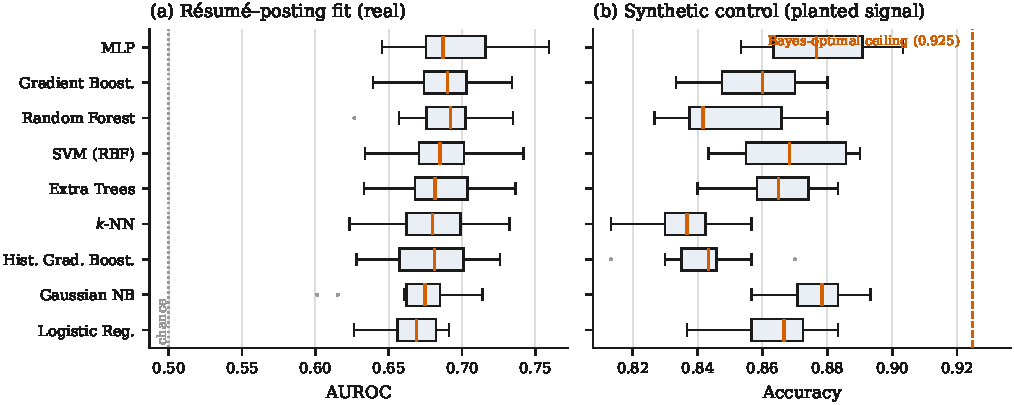
\includegraphics[width=\textwidth]{fig1_convergence_and_power.pdf}
\caption{Per-fold distributions over ten grouped folds. \textbf{(a)} The nine
models on the real résumé--posting task; boxes overlap almost completely.
\textbf{(b)} The same nine models, same folds, same code path, on the synthetic
control with planted signal, against its Bayes-optimal ceiling. Models appear in
the same order in both panels --- the order of panel (a) --- so vertical position
is comparable across panels. The contrast between the panels is the paper's power
analysis: an instrument that reports no difference in (a) is shown in (b) to be
capable of reporting one.}
\label{fig:power}
\end{figure*}

\begin{table*}[t]
\centering\tabfont
\caption{Nine classifiers on résumé--posting fit, 10-fold \texttt{GroupKFold} by
posting, engineered relational features (R2). Efficiency columns are per-fold
means.}
\label{tab:main}
\begin{tabular}{lcccrrrr}
\toprule
Model & AUROC & Accuracy & Macro F1 & ECE & Fit (s) & Latency ($\mu$s/row) & Size (KB) \\
\midrule
MLP                     & \textbf{0.696 $\pm$ 0.031} & 0.634 $\pm$ 0.021 & 0.658 $\pm$ 0.038 & 0.057 & 0.44 & 0.5 & 74.7 \\
Gradient boosting       & 0.689 $\pm$ 0.028 & \textbf{0.636 $\pm$ 0.024} & 0.655 $\pm$ 0.041 & 0.047 & 2.44 & 1.9 & 393.3 \\
Random forest           & 0.688 $\pm$ 0.030 & 0.628 $\pm$ 0.026 & 0.647 $\pm$ 0.042 & 0.047 & 0.59 & 88.2 & 24{,}732.6 \\
SVM (RBF)               & 0.686 $\pm$ 0.028 & 0.635 $\pm$ 0.023 & 0.651 $\pm$ 0.039 & 0.053 & 4.64 & 195.0 & 526.8 \\
Extra trees             & 0.685 $\pm$ 0.030 & 0.632 $\pm$ 0.026 & 0.641 $\pm$ 0.044 & \textbf{0.046} & 0.39 & 84.9 & 63{,}415.9 \\
$k$-NN                  & 0.680 $\pm$ 0.031 & 0.628 $\pm$ 0.029 & 0.639 $\pm$ 0.041 & 0.057 & 0.01 & 35.5 & 1{,}272.8 \\
Hist.\ gradient boosting & 0.679 $\pm$ 0.029 & 0.626 $\pm$ 0.020 & 0.643 $\pm$ 0.037 & 0.057 & 0.41 & 7.3 & 591.8 \\
Gaussian NB             & 0.667 $\pm$ 0.033 & 0.620 $\pm$ 0.027 & 0.633 $\pm$ 0.051 & 0.117 & 0.00 & 0.3 & 1.1 \\
Logistic regression     & 0.665 $\pm$ 0.022 & 0.616 $\pm$ 0.020 & 0.637 $\pm$ 0.042 & 0.052 & 0.01 & 0.2 & \textbf{0.9} \\
\midrule
\textit{Fixed-threshold baseline} & --- & \textit{0.513 $\pm$ 0.028} & --- & --- & --- & --- & --- \\
\bottomrule
\end{tabular}
\end{table*}

The nine span 0.031 AUROC from best to worst. Every model's standard deviation
across folds is of the same order as that entire spread --- the weakest model's
fold-to-fold variation ($\pm 0.022$) is comparable to its distance from the
strongest (0.031).

The Friedman test rejects the hypothesis that all nine perform identically
($\chi^2 = 38.35$, $p = 6.5 \times 10^{-6}$), so the models are not
interchangeable. But the post-hoc picture in Table~\ref{tab:posthoc} is what
matters for a ranking claim.

\begin{table}[t]
\centering\tabfont
\caption{Top model (MLP) against each other model. Paired Wilcoxon signed-rank
over 10 folds, Holm--Bonferroni corrected for eight comparisons.}
\label{tab:posthoc}
\begin{tabular}{lccc}
\toprule
Comparison & $\Delta$AUROC & Holm-adj.\ $p$ & Sig.\ at 0.05 \\
\midrule
MLP vs gradient boosting        & $+0.007$ & 0.262 & no \\
MLP vs random forest            & $+0.008$ & 0.262 & no \\
MLP vs extra trees              & $+0.010$ & 0.193 & no \\
MLP vs hist.\ gradient boosting & $+0.016$ & 0.078 & no \\
MLP vs SVM (RBF)                & $+0.009$ & 0.016 & yes \\
MLP vs $k$-NN                   & $+0.016$ & 0.049 & yes \\
MLP vs Gaussian NB              & $+0.029$ & 0.016 & yes \\
MLP vs logistic regression      & $+0.031$ & 0.016 & yes \\
\bottomrule
\end{tabular}
\end{table}

The leading model is \textbf{statistically indistinguishable from all four tree
ensembles}. It separates only from the linear, probabilistic, instance-based, and
kernel baselines, and even there the largest effect is three AUROC points. A
study that reported only the ranked table would license the claim ``the MLP is
the best model for résumé--job fit.'' The significance analysis does not support
it.

Note also the non-monotonicity between metrics: the MLP leads on AUROC while
gradient boosting leads on accuracy, and extra trees leads on calibration. Which
model ``wins'' depends on which column is placed first.

\subsection{The protocol has power}
\label{sec:power}

Run through the identical protocol, the synthetic control separates the same nine
models decisively (Table~\ref{tab:synth}, Figure~\ref{fig:power}b).

\begin{table}[t]
\centering\tabfont
\caption{The same nine models and the same ten-fold grouped protocol on the
synthetic control. Bayes-optimal accuracy is 0.925 by construction.}
\label{tab:synth}
\begin{tabular}{lccc}
\toprule
Model & Accuracy & AUROC & Macro F1 \\
\midrule
MLP                      & \textbf{0.878 $\pm$ 0.017} & \textbf{0.920 $\pm$ 0.013} & 0.862 $\pm$ 0.015 \\
Gaussian NB              & 0.876 $\pm$ 0.010 & 0.916 $\pm$ 0.013 & 0.859 $\pm$ 0.010 \\
SVM (RBF)                & 0.869 $\pm$ 0.017 & 0.914 $\pm$ 0.013 & 0.852 $\pm$ 0.016 \\
Extra trees              & 0.864 $\pm$ 0.013 & 0.916 $\pm$ 0.014 & 0.844 $\pm$ 0.012 \\
Logistic regression      & 0.864 $\pm$ 0.014 & 0.913 $\pm$ 0.013 & 0.847 $\pm$ 0.015 \\
Gradient boosting        & 0.859 $\pm$ 0.014 & 0.914 $\pm$ 0.014 & 0.842 $\pm$ 0.013 \\
Random forest            & 0.849 $\pm$ 0.017 & 0.912 $\pm$ 0.014 & 0.828 $\pm$ 0.019 \\
Hist.\ gradient boosting & 0.842 $\pm$ 0.014 & 0.904 $\pm$ 0.013 & 0.822 $\pm$ 0.018 \\
$k$-NN                   & 0.836 $\pm$ 0.012 & 0.900 $\pm$ 0.013 & 0.806 $\pm$ 0.013 \\
\midrule
\textit{Bayes-optimal ceiling} & \textit{0.925} & --- & --- \\
\bottomrule
\end{tabular}
\end{table}

Friedman $\chi^2 = 55.42$, $p = 3.7 \times 10^{-9}$ --- three orders of magnitude
more decisive than on the real task, on the same number of folds and models. The
best model recovers 94.9\% of the achievable accuracy, confirming the models are
competently configured rather than crippled.

The comparison between Table~\ref{tab:main} and Table~\ref{tab:synth} is the
argument. Identical folds, identical models, identical code: when learnable
signal is present the protocol resolves it clearly, and when applied to the
résumé task it does not. \textbf{The null result in \S\ref{sec:converge} is a
property of the task, not a limitation of the study.}

One incidental observation deserves recording because it cuts against an
expectation we held before running it. We inserted interaction and quadratic
terms specifically so that models capable of representing non-linear structure
would separate from linear ones, and predicted that logistic regression and naive
Bayes would trail. They did not: Gaussian NB places second and logistic
regression fifth, both above three tree ensembles. The linear component of the
planted signal is strong enough that the non-linear terms shift the ranking
without partitioning it by family. We report this rather than retuning the
generative process, because tuning a control until it produces the expected
ordering is the point at which a control stops being one.

\subsection{Where the ceiling is}
\label{sec:ablation}

Holding the protocol and the folds fixed and varying only the representation
localises the limitation.

\begin{figure}[t]
\centering
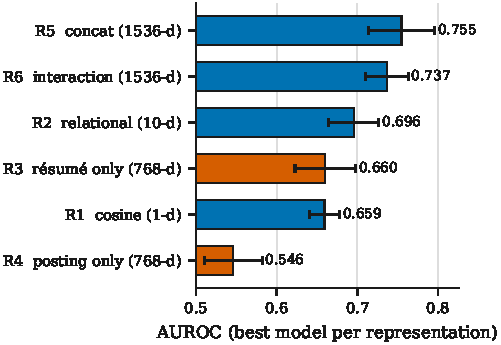
\includegraphics[width=\columnwidth]{fig2_representation_ablation.pdf}
\caption{Best AUROC per representation, identical folds throughout. Highlighted
bars are the one-sided probes, which cannot be performing matching: R3 never sees
the job posting, R4 never sees the résumé. R3 reaches the level of the
single-cosine baseline; R4 sits near chance.}
\label{fig:ablation}
\end{figure}

\begin{table}[t]
\centering\tabfont
\caption{Representation ablation. Identical folds throughout; best of
$\{$logistic regression, random forest, MLP$\}$ per representation.}
\label{tab:ablation}
\begin{tabular}{llcc}
\toprule
Representation & Best model & AUROC & Accuracy \\
\midrule
R5 concat $[r;j]$          & MLP & \textbf{0.755 $\pm$ 0.041} & \textbf{0.681 $\pm$ 0.045} \\
R6 interaction             & RF  & 0.737 $\pm$ 0.026 & 0.661 $\pm$ 0.032 \\
R2 engineered relational   & MLP & 0.696 $\pm$ 0.031 & 0.634 $\pm$ 0.021 \\
\textbf{R3 résumé only}    & RF  & \textbf{0.660 $\pm$ 0.037} & 0.613 $\pm$ 0.027 \\
R1 cosine similarity       & LR  & 0.659 $\pm$ 0.019 & 0.613 $\pm$ 0.023 \\
\textbf{R4 posting only}   & MLP & \textbf{0.546 $\pm$ 0.036} & 0.531 $\pm$ 0.026 \\
\midrule
\textit{Résumé-identity lookup} & --- & --- & \textit{0.609 $\pm$ 0.028} \\
\textit{Fixed-threshold baseline} & --- & --- & \textit{0.513 $\pm$ 0.028} \\
\bottomrule
\end{tabular}
\end{table}

Three readings, in ascending order of consequence.

\textbf{Richer representations do help --- so the engineered features were not
optimal.} R6 exceeds R2 by 0.041 AUROC and R5 exceeds it by 0.059. Ten hand-built
relational features leave signal on the table relative to the full embedding
pair. This partially exonerates the algorithms: the ceiling in
\S\ref{sec:converge} is a ceiling \emph{at that representation}, not an absolute
one.

\textbf{But the ordering tracks résumé access, not relational richness.} R5, plain
concatenation, is the best representation in the study --- better than R6, the
encoding purpose-built for relational tasks. Concatenation's distinguishing
property is not that it captures the relation better; it is that it preserves
each side intact, and therefore permits a model to recognise the résumé. The
representation that most enables memorisation wins.

\textbf{And the two one-sided probes are starkly asymmetric.} A model that never
sees the job posting reaches \textbf{0.660 AUROC} --- statistically
indistinguishable from the single-cosine baseline (0.659), and within 0.036 of
the full engineered relational model. A model that never sees the résumé reaches
\textbf{0.546}, barely above chance. A featureless lookup table that memorises
each résumé's majority label and ignores the posting entirely achieves 0.609
accuracy, against the best model's 0.681.

The asymmetry has a mechanical explanation that is itself the point. Under
grouping by posting, résumés recur between training and test folds while postings
do not --- so R3 can memorise and R4 cannot. That is precisely the recurrence
channel the dataset's own split leaves open, and R3 measures what is reachable
through it. \S\ref{sec:robust} closes the channel by grouping on résumés instead,
and finds performance does not fall --- so the channel is available but not
load-bearing.

\paragraph{A reading to resist.}
The natural inference from Table~\ref{tab:ablation} --- and the one we drew before
testing it --- is that the benchmark's labels are not relational, and that the
apparent performance is memorisation end to end. Table~\ref{tab:ablation} cannot
support that inference, because a pooled metric cannot distinguish a model that
ranks résumés from one that ranks matches: both raise AUROC, and R3 establishes
only that the first is \emph{sufficient} to reach 0.660, not that the second is
absent. \S\ref{sec:matching} measures the second directly, and finds it present.

\subsection{Isolating matching from résumé quality}
\label{sec:matching}

A pooled metric rewards two distinct capabilities and cannot separate them. A
model that knows which \emph{résumés} tend to be labelled fit will score well, and
so will a model that knows which \emph{postings} a given résumé fits. Only the
second is matching. \S\ref{sec:ablation} established that the first is sufficient
to reach 0.660 AUROC; it says nothing about whether the second is present.

\paragraph{Decomposing the label.}
Total label variance (0.25, by construction of the balanced sample) splits into a
between-résumé component --- some résumés are labelled fit more often than others
--- and a within-résumé component, where the same résumé's label changes with the
posting. Only the second is relational.

\begin{table}[h]
\centering\tabfont
\caption{Variance decomposition of the binarised label.}
\label{tab:variance}
\begin{tabular}{lcc}
\toprule
Component & Variance & Share \\
\midrule
Between-résumé & 0.0485 & 19.4\% \\
\textbf{Within-résumé} & \textbf{0.2015} & \textbf{80.6\%} \\
\bottomrule
\end{tabular}
\end{table}

502 of 643 résumés (78\%) carry a label that varies across the postings they
appear with. \textbf{The labels are predominantly relational}, and the majority of
the variance is in principle available only to a model that performs matching.
This alone refutes the hypothesis that the benchmark measures résumé quality and
nothing else.

\paragraph{The within-résumé ranking test.}
To measure whether models access that variance, we restrict evaluation to pairs
of rows sharing a résumé, one positive and one negative, and ask whether the
model assigns the positive posting the higher probability. Because both items of
a pair carry the same résumé, every résumé-level property --- identity, quality,
base rate, verbosity, seniority --- cancels exactly. Chance is 0.5 by
construction. Ties count as one half, following the standard AUROC convention.
For contrast we compute the same statistic over pairs drawn from \emph{different}
résumés, where résumé-level information is fully usable.

\begin{figure}[t]
\centering
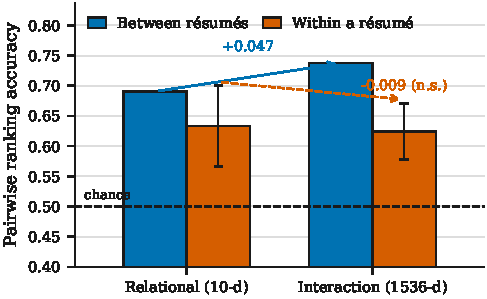
\includegraphics[width=\columnwidth]{fig3_matching_isolation.pdf}
\caption{Pairwise ranking accuracy, chance $= 0.5$. Moving from the engineered
features to the 1536-dimensional interaction encoding raises between-résumé
ranking by 0.047 while leaving within-résumé matching unchanged ($-0.009$,
$p = 0.445$). Error bars are standard deviations across the ten folds. This is
the decoupling the paper reports: the pooled metric moved because the blue bar
moved.}
\label{fig:matching}
\end{figure}

\begin{table}[t]
\centering\tabfont
\caption{Pairwise ranking accuracy. Random forest, identical folds, chance
$= 0.5$. Within-résumé values are pooled over folds; $\pm$ is the standard
deviation across the ten per-fold values.}
\label{tab:matching}
\begin{tabular}{lccc}
\toprule
Representation & Between & Within & Binomial $p$ \\
\midrule
Relational (10-d)     & 0.6905 & \textbf{0.6333 $\pm$ 0.067} & $3.8 \times 10^{-66}$ \\
Interaction (1536-d)  & \textbf{0.7372} & 0.6240 $\pm$ 0.047 & $2.0 \times 10^{-57}$ \\
\bottomrule
\end{tabular}
\smallskip
\caption*{\tabfont Within-résumé pairs: 4{,}112 in both rows. Per-fold $t$-test
against chance: $t = 6.05$, $p = 1.9 \times 10^{-4}$ (relational); $t = 7.96$,
$p = 2.3 \times 10^{-5}$ (interaction).}
\end{table}

\textbf{Models do match.} Both representations rank within-résumé pairs well above
chance, by every test we applied --- pooled binomial across 4{,}112 pairs and a
per-fold $t$-test that treats each fold as one observation. The effect is large
and it is not an artifact of pooling. A model given a single résumé and two
postings picks the fitting one roughly 63\% of the time. Whatever else is true of
this benchmark, it is not empty.

\textbf{But the pooled gain does not come from matching.} Compare the two rows.
Moving from the ten engineered features to the 1536-dimensional interaction
encoding raises between-résumé ranking by \textbf{$+0.047$} and pooled AUROC by
\textbf{$+0.041$} (Table~\ref{tab:ablation}), while within-résumé matching changes
by \textbf{$-0.009$}, which a paired Wilcoxon test over the ten per-fold values
does not distinguish from zero ($p = 0.445$). We state this as \emph{the gain does
not transfer}, not as \emph{matching degrades}: the data support the absence of an
improvement, not the presence of a loss.

This is the paper's central measurement. The representation change that a
leaderboard would record as a clear improvement bought a better ordering of
résumés against each other and left the model's ability to tell which posting
suits a candidate exactly where it was. The pooled metric reports the sum of two
capabilities and moved because one of them moved; nothing in that metric reveals
which.

\paragraph{The diagnostic generalises.}
Nothing in the construction is specific to résumés. Any benchmark whose instances
are (entity, item) pairs and in which entities recur --- candidate--job,
patient--treatment, user--item, student--question, query--document --- admits the
same test: condition on the entity, rank within it, compare against the pooled
number. It needs no extra labels and one pass over predictions already computed.
Where the within-entity and pooled numbers diverge, the pooled number is
measuring something other than the advertised capability, and reporting both
makes the difference visible at negligible cost.

\subsection{Robustness}
\label{sec:robust}

Two objections bear directly on the interpretation above, and both are testable.
Neither survives, and one of them fails in a direction we did not predict.

\paragraph{Objection 1: the protocol still permits résumé leakage.}
Grouping by posting holds postings out but leaves résumés shared between folds.
We hold the features and model fixed (engineered relational, random forest) and
vary only the splitting scheme.

\begin{table}[h]
\centering\tabfont
\caption{Split-scheme comparison. Identical features, identical model, 10 folds
throughout.}
\label{tab:splits}
\begin{tabular}{llcc}
\toprule
Scheme & Held out & AUROC & Accuracy \\
\midrule
S1 $k$-fold, no grouping & nothing & \textbf{0.7137 $\pm$ 0.016} & 0.6485 \\
S3 GroupKFold by résumé  & test résumés & 0.7032 $\pm$ 0.031 & 0.6449 \\
S2 GroupKFold by posting & test postings & 0.6894 $\pm$ 0.016 & 0.6331 \\
\bottomrule
\end{tabular}
\end{table}

\textbf{The naive protocol inflates, modestly.} S1 --- the ungrouped scheme a
conventional bake-off would use --- scores 0.024 AUROC above the posting-grouped
protocol we adopt. A study reporting S1 would overstate generalisation to unseen
postings by roughly that margin. The effect is real and worth controlling, and it
is smaller than the leakage literature's more dramatic
cases~\cite{kapoor2023leakage}.

\textbf{Closing the résumé channel does not collapse performance --- it raises
it.} We expected S3, in which no test résumé has been seen during training, to
fall sharply if the model's apparent skill were résumé recognition. It scores
0.014 \emph{above} S2. A strong-memorisation account predicts the opposite sign
and is refuted.

The ordering instead tracks \textbf{which side of the pair is novel}. S2 confronts
the model with postings it has never seen; S3 with résumés it has never seen but
postings it has. Generalising to a new posting is the harder problem of the two.
That is worth stating in its own right: in deployment, every new job requisition
is an S2 instance, so S2 is the protocol that reports the number a practitioner
would actually experience --- which is why we adopted it, and it is the most
pessimistic of the three.

This also refines \S\ref{sec:ablation}. R3 established that the résumé side
\emph{alone} supports 0.660 AUROC. S3 shows that relational features reach 0.703
with the résumé side entirely held out. Memorisation is available and worth
something; it is not load-bearing, and the ``shortcut'' reading of
Table~\ref{tab:ablation} that we warned against there is now excluded from two
independent directions.

\paragraph{Objection 2: binarising the three-class label destroyed the relational
signal.}
\texttt{Potential Fit} is a fuzzy middle class, and collapsing it into the
positive class could plausibly blur the boundary that carries the matching
information.

\begin{table}[h]
\centering\tabfont
\caption{Label-granularity comparison. GroupKFold by posting throughout.}
\label{tab:labels}
\begin{tabular}{lrcc}
\toprule
Formulation & Rows & AUROC & Accuracy \\
\midrule
L1 Good + Potential vs No Fit & 8{,}000 & \textbf{0.6894 $\pm$ 0.016} & 0.6331 \\
L2 Good vs No Fit, Potential dropped & 6{,}000 & 0.6810 $\pm$ 0.050 & 0.6497 \\
L3 three-class, macro one-vs-rest & 8{,}000 & 0.6518 & --- \\
\quad --- vs-rest: No Fit & & 0.6894 $\pm$ 0.016 & 0.6331 \\
\quad --- vs-rest: Good Fit & & 0.6365 $\pm$ 0.068 & 0.6267 \\
\quad --- vs-rest: Potential Fit & & 0.6296 $\pm$ 0.029 & 0.5918 \\
\bottomrule
\end{tabular}
\end{table}

The cleanest available contrast --- Good Fit against No Fit with the ambiguous
class removed entirely --- does \textbf{not} exceed the binarisation we use (0.6810
vs 0.6894), and its fold-to-fold variance triples. The three-class macro AUROC is
lower still, and the \texttt{Potential Fit} class is the hardest of the three to
separate from the rest. Binarisation is not concealing signal; the middle class
carries information that discarding it loses.

\paragraph{A note on sample size.}
This experiment uses all 8{,}000 rows, which are already balanced 4{,}000/4{,}000
under the binarisation, with class weights handling the residual imbalance in L2
and L3. The main experiments balance within each of the dataset's own splits and
so retain 7{,}910. The two pipelines agree where they overlap: S2/L1 here reaches
0.6894, against the random forest's 0.688 in Table~\ref{tab:main}.

\paragraph{Objection 3: the models were not tuned.}
This is the most serious of the three, because it attacks \S\ref{sec:converge}
directly. We ran a nested cross-validation designed so that it \emph{could}
refute the paper's central claim: if tuning pulls one model clear of the others,
``statistically indistinguishable'' fails.

The outer loop is the same ten folds used throughout. Inside each outer training
fold, a 3-fold \texttt{GroupKFold} (again by posting) selects among \textbf{eight
configurations per model, an identical budget for every model} --- an unequal
budget would compare search effort rather than algorithms. The selected
configuration is refit on the full outer-training fold and scored once on the
untouched outer-test fold, so no test row influences any selection.

\begin{table}[h]
\centering\tabfont
\caption{Equal-budget nested hyper-parameter search. Tuned AUROC is mean $\pm$ sd
over the ten outer folds; untuned values are from Table~\ref{tab:main}.}
\label{tab:tuned}
\begin{tabular}{lccr}
\toprule
Model & Tuned AUROC & Untuned & $\Delta$ \\
\midrule
MLP                      & \textbf{0.6938 $\pm$ 0.026} & 0.6958 & $-0.0020$ \\
SVM (RBF)                & 0.6913 $\pm$ 0.027 & 0.6863 & $+0.0050$ \\
Gradient boosting        & 0.6902 $\pm$ 0.031 & 0.6891 & $+0.0011$ \\
$k$-NN                   & 0.6874 $\pm$ 0.029 & 0.6797 & $\mathbf{+0.0077}$ \\
Random forest            & 0.6862 $\pm$ 0.029 & 0.6881 & $-0.0019$ \\
Hist.\ gradient boosting & 0.6835 $\pm$ 0.030 & 0.6795 & $+0.0040$ \\
Extra trees              & 0.6826 $\pm$ 0.029 & 0.6855 & $-0.0029$ \\
Gaussian NB              & 0.6671 $\pm$ 0.033 & 0.6671 & $+0.0000$ \\
Logistic regression      & 0.6621 $\pm$ 0.022 & 0.6647 & $-0.0026$ \\
\bottomrule
\end{tabular}
\end{table}

\textbf{Tuning does not rescue any model.} The largest gain across all nine is
$+0.0077$ ($k$-NN) and three models are marginally worse tuned than untuned,
which is ordinary nested-CV selection noise. No model moves enough to change its
position materially.

\textbf{And it makes the field more homogeneous, not less.} The best-to-worst
spread is essentially unchanged (0.0311 untuned $\rightarrow$ 0.0317 tuned), but
the \emph{significance} structure contracts. Friedman still rejects overall
($\chi^2 = 41.28$, $p = 1.8 \times 10^{-6}$), yet after Holm correction the tuned
leader separates from only \textbf{two} of eight comparisons --- Gaussian NB
($p = 0.016$) and logistic regression ($p = 0.016$) --- where the untuned leader
separated from four. The two models that were significantly behind and gained
most from tuning, SVM and $k$-NN, are no longer distinguishable from the leader.

This converts the argument in \S\ref{sec:threats} into a measurement.
Equal-budget tuning leaves the ranking substantively unchanged, leaves the spread
unchanged, and \emph{weakens} rather than strengthens the case that any model is
best. The convergence in \S\ref{sec:converge} is not an artifact of unturned
dials.

\subsection{Accuracy and cost are decoupled}
\label{sec:efficiency}

\begin{figure}[t]
\centering
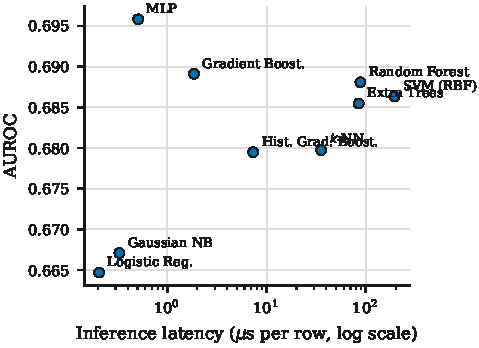
\includegraphics[width=\columnwidth]{fig4_efficiency_pareto.pdf}
\caption{AUROC against inference latency (log scale). The frontier is nearly
flat: three orders of magnitude of latency buy 0.031 AUROC, most of which is not
statistically resolvable.}
\label{fig:efficiency}
\end{figure}

The efficiency columns of Table~\ref{tab:main} support a conclusion independent of
the accuracy analysis. Across the nine models, inference latency spans
\textbf{0.2 to 195.0 $\mu$s per row} --- a factor of roughly 1{,}000 --- and
serialised model size spans \textbf{0.9 KB to 63.4 MB}, a factor of about
70{,}000. Predictive quality spans 0.031 AUROC.

The two are not merely weakly related; they are close to unrelated. Logistic
regression is the smallest model in the study by a factor of 27{,}000 and the
fastest by a factor of 975, and sits 0.031 AUROC below the leader --- a gap that
is significant but small. Extra trees occupies 63 MB to land mid-table. The RBF
SVM is the slowest model at inference and ranks fourth.

For a deployment that must score candidates interactively, this is the operative
finding. The cost--quality frontier on this task is nearly flat, so the rational
choice is the cheapest model that is not significantly worse --- which here is a
kilobyte of logistic-regression coefficients, not a 64-megabyte forest.

\subsection{More data does not close the gap}

\begin{figure}[t]
\centering
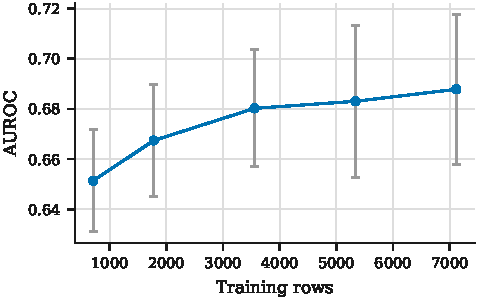
\includegraphics[width=\columnwidth]{fig5_learning_curve.pdf}
\caption{Learning curve for the engineered representation with a random forest,
over the same ten folds. The curve flattens well below any useful operating
point.}
\label{fig:curve}
\end{figure}

\begin{table}[h]
\centering\tabfont
\caption{Learning curve on R2 with a random forest, same folds.}
\label{tab:curve}
\begin{tabular}{lrc}
\toprule
Training fraction & $\approx$ rows & AUROC \\
\midrule
10\%  &   712 & 0.6514 \\
25\%  & 1{,}779 & 0.6674 \\
50\%  & 3{,}559 & 0.6802 \\
75\%  & 5{,}339 & 0.6830 \\
100\% & 7{,}119 & 0.6878 \\
\bottomrule
\end{tabular}
\end{table}

Quadrupling the training data from 25\% to 100\% buys 0.0204 AUROC; doubling from
50\% to 100\% buys 0.0076. The curve is flattening well below any useful
operating point. The limitation is not sample size, and collecting more rows of
this kind would not resolve it.

\section{Discussion}

\subsection{What these results establish}

\paragraph{Algorithm choice is not the bottleneck at a fixed representation.}
Nine classifiers spanning six families span 0.031 AUROC, and the leader is
statistically indistinguishable from four of them (\S\ref{sec:converge}). The
synthetic control (\S\ref{sec:power}) rules out the interpretation that the
protocol simply could not tell them apart. For practitioners, the operational
reading is that effort spent selecting among these families on this task is
effort not spent on the thing that does move the number.

\paragraph{Representation matters roughly twice as much as algorithm.}
Changing the representation while holding the model family fixed moves AUROC by
0.059 (R2 $\rightarrow$ R5); changing the algorithm while holding the
representation fixed moves it by 0.031 across all nine models, with most of that
range not statistically resolvable. This is consistent with the broader
tabular-learning literature~\cite{grinsztajn2022tabular} and unsurprising in
itself. It is worth stating precisely because the bake-off format invites the
opposite allocation of effort.

\paragraph{The benchmark contains genuine relational signal, and models capture
part of it.}
80.6\% of label variance is within-résumé, and within-résumé ranking runs well
above chance at 0.633 ($p < 10^{-65}$, and $p < 10^{-3}$ by the conservative
per-fold test). Independently, holding every test résumé out of training does not
reduce performance (\S\ref{sec:robust}) --- it slightly increases it --- which a
memorisation account cannot produce. Two experiments designed to expose a
shortcut instead established that the underlying task is being partly solved. We
emphasise this because a paper of this genre is prone to overclaiming in the
sceptical direction, and because both results contradicted our own hypothesis.

\paragraph{Generalising to a new posting is harder than generalising to a new
candidate.}
The three splitting schemes order as S1 $>$ S3 $>$ S2 (\S\ref{sec:robust}): the
protocol that withholds postings is the most demanding of the three. This has a
direct deployment reading --- every new job requisition presents the S2 condition
--- and it suggests that reported figures obtained under ungrouped splits
overstate the performance a screening system would show on a newly opened role by
roughly 0.024 AUROC.

\paragraph{Pooled score and matching ability are nonetheless decoupled.}
The representation change worth $+0.041$ pooled AUROC and $+0.047$ between-résumé
ranking produced no measurable within-résumé improvement (\S\ref{sec:matching}).
The two capabilities that the pooled metric sums moved independently, and the
metric could not indicate which one had moved.

\subsection{What they do not establish}

We are not claiming that résumé--posting matching is unlearnable, that this
dataset is unfit for use, or that any specific published result using it is
incorrect --- we have not audited other work's protocols and make no claim about
them. We are also not claiming that the shortcut is a defect introduced by the
dataset's authors: grouping by job description is a reasonable choice, and the
recurrence of résumés across rows is intrinsic to how a résumé--posting corpus is
built. The claim is narrower: on this benchmark, the pooled metric conflates two
capabilities, one of which is far easier to acquire, and nothing in the standard
reporting format reveals the composition.

\subsection{The within-query diagnostic should be routine}

The measurement in \S\ref{sec:matching} costs one pass over predictions that have
already been computed, requires no additional labels, and has a fixed null value
of 0.5 that needs no baseline model to establish. Its diagnostic content is high
precisely because entity-level information cancels exactly rather than
approximately: unlike a controlled feature ablation, there is no residual leakage
to argue about.

Any benchmark whose instances are (entity, item) pairs with recurring entities
admits it --- candidate--job, patient--treatment, user--item, student--question,
query--document. In each case the pooled metric rewards both ``this entity tends
to be positive'' and ``this item suits this entity,'' and in each case only the
second is usually the advertised capability. We suggest reporting the
within-entity statistic alongside the pooled one as a matter of course, and
treating a divergence between them as information rather than as an anomaly to be
explained away.

The general form of the recommendation: \textbf{when a benchmark's instances pair
a recurring entity with a varying item, report the metric conditioned on the
entity.} If the conditioned number is flat while the pooled number rises, the
improvement is in entity ranking, and the leaderboard is not measuring the task.

\subsection{Implications for algorithmic hiring}

Raghavan et al.~\cite{raghavan2020hiring} observed that vendors' choice of
prediction target carries much of the ethical and legal weight in algorithmic
hiring, because downstream fairness analysis is conducted against the stated
target. Our results give that observation a concrete measurement problem.

A model marketed as scoring \emph{fit between a candidate and a role} but whose
measured improvements come from ranking \emph{candidates against one another} is,
functionally, a general-purpose candidate ranker carrying a role-specific label.
The distinction is not cosmetic. A fit score is contestable in a specific way ---
a candidate can ask which requirement of this posting they were judged not to
meet. A latent résumé-quality score offers no such handle, generalises across
every posting the system serves, and reproduces whatever the training labels
encoded about what a good résumé looks like. Those are materially different
artifacts with materially different disparate-impact profiles, and the difference
is invisible in a pooled AUROC.

We are not in a position to say what any deployed system does; we have measured
one public benchmark. What we can say is that the standard reported metric would
not distinguish the two cases, and that a within-query statistic would. For a
domain under active regulatory attention, a diagnostic that separates ``ranks
people'' from ``ranks matches'' at negligible cost seems worth adopting.

\subsection{On reporting a hypothesis we refuted}

We designed \S\ref{sec:matching} to confirm that this benchmark's labels were not
relational, having been led there by the résumé-only probe reaching 87\% of the
best model's AUROC. The test refuted the hypothesis cleanly, and we have kept the
sequence visible rather than presenting the surviving result as though it had
been the plan.

The methodological point is not about candour for its own sake. A diagnostic
whose value is that it can distinguish two hypotheses is only demonstrated to
have that value when it actually overturns one. Had we reported only the final
claim, the within-query test would read as a confirmatory statistic; the fact
that it contradicted the conclusion we expected is the strongest available
evidence that it measures something the pooled metric does not.

\section{Threats to Validity}
\label{sec:threats}

\paragraph{A single dataset.}
Every result here concerns one benchmark. We do not claim that our conclusions
generalise beyond it, and replication on an independent résumé--fit corpus
remains the most valuable extension of this work. As \S\ref{sec:noreplication}
documents, we attempted that replication and found no public corpus that
qualifies: the most-downloaded alternatives are derivatives of the corpus under
study --- one shares 100\% of its documents --- and the genuinely independent
candidates pair each résumé with exactly one posting, which makes the
within-query statistic undefined rather than merely noisy. The limitation is real
and we do not minimise it; we record that it presently binds on data availability
rather than on effort.

\paragraph{Encoder choice and truncation.}
Documents are embedded with a single 768-d encoder and truncated to 2{,}000
characters for embedding. A stronger encoder, or a cross-encoder that attends
jointly over both documents, could extract relational signal that ours cannot.
Two considerations bound this threat. First, the résumé-only probe (R3) uses the
\emph{same} encoder, so its near-parity with the full relational model cannot be
explained by encoder weakness --- a weak encoder would degrade both. What must be
explained is the \emph{asymmetry} between R3 and R4, which is a property of the
split and the labels, not of the embedding. Second, token-level features read
untruncated text, so the truncation affects only the embedding-derived
components.

\paragraph{Hyper-parameter tuning.}
The headline comparison runs models at fixed modest settings. We tested whether
that matters with an equal-budget nested search (\S\ref{sec:robust}, Objection 3)
and it does not: the largest gain across nine models is $+0.0077$ AUROC, the
best-to-worst spread is unchanged ($0.0311 \rightarrow 0.0317$), and the tuned
leader separates significantly from fewer models than the untuned one. The
residual threat is that a substantially larger search than eight configurations
per model, or a better-chosen grid, could yet find something we did not. We
regard that as unlikely to change a conclusion \S\ref{sec:ablation} shows is
representational rather than algorithmic, but it is not excluded.

\paragraph{Class balancing by downsampling.}
We discard majority-class rows to make 50\% the exact random baseline. This costs
data and could in principle alter the learnable structure; the retained sample is
large relative to the flattening point of the learning curve in
Table~\ref{tab:curve}.

\paragraph{The synthetic control is a control, not a simulation.}
Its generative process is not a model of résumé screening and its ceiling is an
artifact of a flip rate we chose. It licenses exactly one inference --- that the
protocol can detect differences of this magnitude at this sample size --- and
nothing about résumé data.

\paragraph{The within-résumé test runs on a subset.}
It requires a résumé to appear with both a positive and a negative posting
\emph{inside the same test fold}, which yields 4{,}112 pairs across the ten folds
and excludes résumés whose postings did not co-occur in a fold. Those résumés may
differ systematically from the included ones. Per-fold variation is also
substantial ($\pm 0.067$ for the engineered features, with one fold at 0.481),
which is why we report both a pooled binomial test and a conservative per-fold
$t$-test, and why the R2-versus-R6 comparison is reported as a null rather than
as a difference. We additionally cap the pairs contributed by any one résumé at
40 so that a prolific résumé cannot dominate the statistic.

\paragraph{A negative result about transfer is not a proof of no transfer.}
\S\ref{sec:matching} shows no measurable within-résumé gain from a representation
change worth $+0.041$ pooled AUROC. With ten folds and this variance, a true
within-résumé improvement of one or two points would likely have gone undetected.
The claim is that the pooled gain is not \emph{predominantly} matching
improvement, not that matching improvement is exactly zero.

\section{Conclusion}

We set out to determine which of nine classifiers is best for résumé--job-description
fit, and found that the question is not answerable on this benchmark and not the
useful question to ask of it. Nine algorithms spanning six families converge into
a three-point AUROC band in which the leader is statistically indistinguishable
from every tree ensemble tested. A synthetic control run through the identical
protocol separates the same nine decisively, so the convergence is a property of
the task rather than of the study.

Asking what does move the number produced a more useful answer than the ranking
would have. A model that never sees the job posting reaches 87\% of the best
model's AUROC, and the highest-scoring representation in the study is plain
concatenation --- the encoding that most preserves each document intact and
therefore most enables the model to recognise a résumé it has seen.

That evidence pointed toward a strong conclusion, that the benchmark's labels
were not relational at all, and a direct test refuted it. Four-fifths of the label
variance is within-résumé, and models rank within-résumé pairs well above chance.
The task is real and the models partly solve it.

What survives is a decoupling. A representation change worth $+0.041$ pooled
AUROC and $+0.047$ between-résumé ranking delivered no measurable change in
within-résumé matching. The pooled metric reports the sum of two capabilities ---
ranking candidates, and matching candidates to roles --- and moved because the
easier one moved. Nothing in the reported number distinguishes the two, and a
leaderboard built on it will reward the shortcut whenever the shortcut is
cheaper, which here it is.

The remedy is inexpensive. Conditioning the metric on the recurring entity
cancels entity-level information exactly, costs one pass over existing
predictions, needs no additional labels, and has a null value of 0.5 that
requires no baseline to establish. Where the conditioned number tracks the pooled
one, the pooled one is reporting what its name suggests. Where they diverge --- as
here --- the divergence is the finding.

For a task whose deployed form decides who is considered for work, the difference
between a system that ranks matches and one that ranks people is not a
technicality, and it should not require a dedicated study to detect.

\bibliographystyle{plain}
\bibliography{references}

\appendix

\section{Reproduction}
\label{sec:repro}

Every experiment is a single command from \texttt{service/}, deterministic at
seed 100 given a fixed embedding cache.

\paragraph{On the embedding cache.}
Document embeddings are cached by content hash in
\texttt{service/ml/resume\_fit/cache/embeddings.json} ($\sim$16\,MB). That file is
\textbf{not} committed --- it is excluded by \texttt{.gitignore} on size grounds ---
so a first run must regenerate it, which requires a local Ollama instance serving
\texttt{nomic-embed-text}. Regeneration touches only the ${\sim}1{,}470$ unique
documents and is a one-off cost. Regenerated embeddings are reproducible only
against the same encoder version, so exact replication of the embedding-derived
features depends on that model being unchanged; all splitting, fitting, and
statistical steps are seeded and exactly reproducible.

\begin{table}[h]
\centering\tabfont
\caption{Reproduction commands.}
\begin{tabular}{lll}
\toprule
Experiment & Section & Command \\
\midrule
Nine-algorithm comparison & \ref{sec:converge} & \texttt{python -m ml.resume\_fit.train\_benchmark} \\
Synthetic positive control & \ref{sec:power} & \texttt{python -m ml.synthetic\_benchmark} \\
Representation ablation & \ref{sec:ablation} & \texttt{python -m ml.resume\_fit.ablation} \\
Matching isolation & \ref{sec:matching} & \texttt{python -m ml.resume\_fit.matching\_isolation} \\
Split and label robustness & \ref{sec:robust} & \texttt{python -m ml.resume\_fit.robustness} \\
Nested tuning check & \ref{sec:robust} & \texttt{python -m ml.resume\_fit.tuned\_benchmark} \\
Dataset diagnostics & --- & \texttt{python -m ml.resume\_fit.diagnose} \\
Replication-corpus screen & \ref{sec:noreplication} & \texttt{python -m ml.resume\_fit.probe\_datasets} \\
Contamination verification & \ref{sec:noreplication} & \texttt{python -m ml.resume\_fit.verify\_med2425} \\
Figures & all & \texttt{python -m ml.make\_figures} \\
\bottomrule
\end{tabular}
\end{table}

Outputs: per-fold CSVs and JSON reports next to each script; figures in
\texttt{docs/paper/figures/}. \texttt{matplotlib} is required for figures only
and is deliberately absent from \texttt{requirements.txt}, which feeds the
deployed image.

\end{document}
